\section{METHOD}
Up to this point, we formally defined what an attack graph is. In this section, we first look at how the existing components of attack graph generation for computer networks map into a microservice environment and provide a small example (Subsection \ref{chap:mapping}). We then in Subsection \ref{chap:technical} refer to the third party tools that we use to achieve this translation and present an overview of our proposed system with its components: Topology Parser in Subsection \ref{chap:topology_p}, Vulnerability Parser in Subsection \ref{chap:vulnerability_p} and Attack Graph Parser Subsection \ref{chap:attack_graph_p} with the Breath-first Search graph traversal algorithm in Subsection \ref{chap:bfs}. 


%\todo{it is early to put this image here, also long caption, image quality should be enhanced}
\begin{figure}
	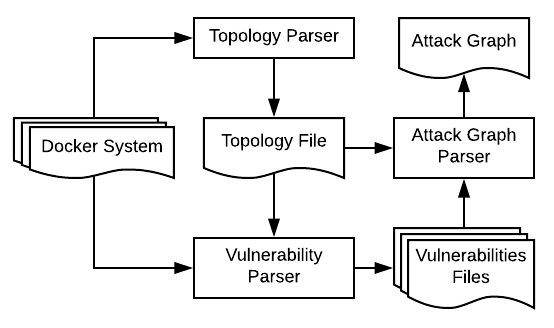
\includegraphics[scale=0.9]{./images/AttackGraphSystem}
	\caption{Our Attack Graph System. The rectangles denote the main components of the system: Topology Parser, Vulnerability Parser and Attack Graph Parser. The arrows describe the flow of the system and the files are the intermediate products.}
	\label{AttackGraphSystem}
\end{figure}

\subsection{Mapping attack graphs from network to microservice perspective}
\label{chap:mapping}

In our work, we try to translate already existing attack graph generation work from computer networks into the microservices ecosystem. In order to do this, we identify the different components and find a compatible replacement that can be used in a microservice architecture. In this subsection, we start first by shortly introducing a famous microservice framework(Docker) and some of its terminology. We then modify the attack graph concepts mentioned above for our use-case(nodes, edges, privilege levels, pre- and postconditions). In the end, we see how this translation works in practice by demonstrating a small example.

Docker is one of the most popular and used microservice frameworks currently available. In Docker, a distinction is being made between the terms image, container and service. An image is an executable package that includes everything needed to run an application, a container is a runtime instance of an image and service represents a container in production. A service only runs one image, but it codifies the way that image runs, what ports it should use, how many replicas of the container should run so the service has the capacity it needs  \cite{merkel2014docker}. In our work, we treat these terms equally, since we are doing a static and not runtime attack graph analysis.

As mentioned above, nodes and edges are the basic building blocks of an attack graph. Nodes in this attack graph model are represented as a combination of docker images and their respective privilege levels, while edges are connections between node pairs accompanied by the vulnerabilities that are being exploited as descriptors. In order for an attacker to exploit a given vulnerability, certain preconditions have to be met. Once an attacker exploits this vulnerability, he gains the privilege of the target container as a postcondition and an edge is added to the attack graph. Both the pre- and postconditions in this work are transformed from pre- and postcondition rules manually selected and evaluated by experts in existing work \cite{aksu2018automated}. The pre- and postcondition rules use the fields defined by NVD, as well as an occurrence of specific keywords from the CVEs descriptions \cite{booth2013national}.

Privileges play a central role in this attack graph generation. We model the privileges in a hierarchy. The privileges in ascending order are None, VOS(User), VOS(Admin), OS(User) and OS(Admin). VOS means that the privilege is exclusive to a virtual machine, while not affecting the host machine. On the other side, The keyword OS means that the host machine has been compromised. Since VOS are hosted on some machines, and their exploitation does not imply exploitation of the host machine, they are in the lower level of hierarchy \cite{aksu2018automated}. None means that no privilege is obtained, User that only a subset of user level privileges are available, while Admin grants control over the whole system.

In order to show how the attack graph generation works in practice, we present a small example. The example is taken from the Netflix OSS Github repository \cite{netflixoss}. Displayed in Figure \ref{TopologyGraph} is the topology of the example. The topology consists of "Outside" node, "Docker daemon" node and a subset of other nodes. In Figure \ref{AttackGraph} we can see a part of the resulting attack graph. Parts of both graphs have been intentionally omitted to reduce complexity. An example path that an attacker would take could be to first attack the Zuul container by exploiting the CVE-2016-10249 vulnerability and gain USER privilege. Then with this USER privilege, it can exploit the CVE-2015-7554 vulnerability on the same container to gain ADMIN privilege. Once the ADMIN privilege has been obtained on Zuul, the attacker can attack the Eureka container by exploiting CVE-2017-7600 and gain ADMIN privilege. It is important to note that this is not the only path that the attacker can take in order to have ADMIN privileges on Eureka. Another path would be to exploit the CVE-20108-1124 vulnerability while have only USER privilege on Zuul to gain directly ADMIN privileges and then attack the Eureka container. Our attack graph generator shows both paths since it is of an interest to see every possible route in which a container can be compromised.

Our attack graph generator is composed of three main components: Topology Parser, Vulnerability Parser and Attack Graph Parser(Fig. \ref{AttackGraphSystem}). The Topology Parser reads the underlying topology of the system and converts it into to a format needed for our Attack Graph Parser, the Vulnerability Parser generates the vulnerabilities for each of the images and the Attack Graph Parser generates the attack graph from the topology and vulnerabilities files. 

\begin{figure}
	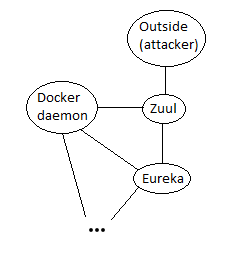
\includegraphics[]{./images/Topology_graph}
	\caption{Example topology graph. The topology graph is a subset of a real topology graph from the Netflix OSS example. Each node denote container(plus Docker Deamon and Outside) and each edge denotes a connection between two containers.}
	\label{TopologyGraph}
\end{figure}

\begin{figure}
	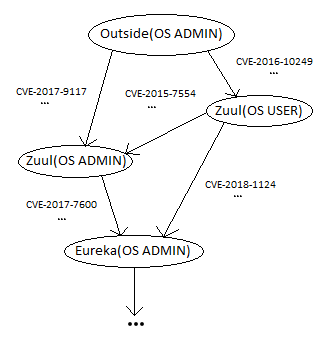
\includegraphics[]{./images/Attack_graph}
	\caption{Example resulting attack graph. This attack graph is a subset of a real attack graph from the Netflix OSS example. Nodes correspond to a pair of container plus privilege, while edges are atomic attacks.}
	\label{AttackGraph}
\end{figure}


In the following subsections, we first have a look into the system requirements, then describe each of the parsers in more detail and finally examine the characteristics of the Breath-first Search graph transversal algorithm.

\subsection{Technical Details}
\label{chap:technical}

Our system is developed for Docker 17.12.1-ce and Docker Compose 1.19.0 \cite{merkel2014docker}. The code is written in Python 3.6, and we use Clair \cite{clair} and Clairctl \cite{clairctl} for vulnerabilities generation.

We developed this system to be used exclusively with a specific version of Docker and Docker-Compose. However, please note that the main algorithm is easily extendable to accommodate other microservice architectures if the appropriate Topology and Vulnerability parsers are provided and conform to the input of the attack graph generator.

\subsection{Topology Parser}
\label{chap:topology_p}

The topology of Docker containers can be described at either runtime or statically by using Docker Compose. In our case, since we are doing static attack graph analysis, we use Docker Compose as our main tool in the beginning. Docker Compose provides us with a docker-compose.yml file which is used for extraction of the topology of the system. However different versions of docker-compose.yml, use different syntax. For example, older versions use the deprecated keyword "link", while newer ones use exclusively "networks", to denote a connection between two containers. In this work, we use the keyword "networks" as an indicator that a connection between two containers exists.

However, in the majority of cases, in order for an application to be useful, it has to communicate with the outside world. This is usually done by using publishing ports. This is the case in both computer networks, as well as in microservice architectures.

Another consideration that we take into account is the privileged access. Some containers require certain privileges over the docker daemon in order to function properly. In docker, this is usually done either by mounting the docker socket or specifying the keyword "privileged" in the docker-compose.yml file. An attacker with access to these containers has also access to the Docker daemon. Once the attacker has access to the docker daemon, he has potential access to the whole microservice system, since every container is controlled and hosted by the daemon.

\begin{algorithm}
	\SetAlgoLined
	\KwData{topology, cont\_expl,
		priv\_acc}
	\KwResult{nodes, edges}
	nodes, edges, passed\_nodes = [], [], [] \\
	queue = Queue() \\
	queue.put("outside" + "ADMIN") \\
	
	\While{! queue.isEmpty()}{
		curr\_node = queue.get() \\
		curr\_cont = get\_cont(curr\_node) \\
		curr\_priv = get\_priv(curr\_node) \\
		neighbours = topology[curr\_cont] \\
		\For{neigh in neighbours}{
			\If{curr\_cont == docker\_host}
			{
				end = neigh + "ADMIN" \\
				create\_edge(curr\_node, end) \\
			}
			\If{neigh == docker\_host and priv\_acc[curr\_cont]}
			{ 	
				end = neigh + "ADMIN" \\
				create\_edge(curr\_node, end) \\
				queue.put(end) \\
				passed\_nodes.add(end)    	
			}
			\If{neigh != outside and neigh != docker\_host}{
				precond = cont\_expl[neigh][precond] \\
				postcond = cont\_expl[neigh][postcond] \\
				\For{vul in vuls}{
					\If{$curr_priv > precond[vul]$}{	
						end = neigh + post\_cond[vul]\\
						create\_edge(curr\_node, end\_node)\\
						\If{end\_node not in passed\_nodes}{
							queue.put(end\_node)\\
							passed\_nodes.add(end\_node)
						}}
					}
				}
			}
			nodes = update\_nodes()\\
			edges = update\_edges() \\
		}
		
		\caption{Breadth-first Search algorithm for generating an attack graph.}
		\label{BFSalgorithm}
	\end{algorithm}
	

	
\subsection{Vulnerability Parser}
\label{chap:vulnerability_p}

In the preprocessing step, we use Clair to generate the vulnerabilities of a given container. Clair is a vulnerability scanner that inspects a docker image and generates its vulnerabilities by providing CVE-ID, description and attack vector for each vulnerability \cite{clair}. An attack vector is an entity that describes which conditions and effects are connected to this vulnerability. The fields in the attack vector as described by the National Vulnerability Database(NVD) \cite{booth2013national} are: Access Vector(Local, Adjacent Network and Network), Access Complexity(Low, Medium, High), Authentication(None, Single, Multiple), Confidentiality Impact(None, Partial, Complete), Integrity Impact(None, Partial, Complete) and Availability Impact(None Partial Complete). Unfortunately, Clair does not provide with a ready to use interface to analyze a docker image. As a result, we use Clairctl \cite{clairctl} in order to analyze a complete docker image.


\subsection{Attack Graph Parser}
\label{chap:attack_graph_p}

After the topology file is extracted and the vulnerabilities for each container are generated, we continue with the attack graph generation. Here, we first preprocess the vulnerabilities and convert them into sets of pre- and postconditions. In order to do this, we match the attack vectors acquired earlier from the vulnerability database and keywords of the descriptions of each vulnerability to generate attack rules. When a subset of attack vector fields and description keywords matches a given rule, we use the pre- or postcondition of that rule. If more than one rule matches, we take the one with the highest privilege level for the preconditions and the lowest privilege level for the postconditions. If no rule matches, we take None as a precondition and ADMIN(OS) as a postcondition. This results in a list of container vulnerabilities with their preconditions and postconditions.

\subsubsection{Breadth-first Search}
\label{chap:bfs}

After the preprocessing step is done, the vulnerabilities are parsed and their pre- and postconditions are extracted. Together with the topology, they are feed into the Breadth-first Search algorithm (BFS).
Breadth-first Search is a popular search algorithm that traverses a graph by looking first at the neighbors of a given node, before diving deeper into the graph. Pseudocode of our modified Breadth-first Search is given in Algorithm \ref{BFSalgorithm}. The algorithm requires a topology and a dictionary of the exploitable vulnerabilities as an input and the output is made up of nodes and edges that make the attack graph. The algorithm first initializes the nodes, edges, queue and the passed nodes. Afterward, it generates the nodes which are a combination of the image name and the privilege level. Then into a while loop, it iterates through every node, checks its neighbors and adds the edges if the conditions are satisfied. If the neighbor was not passed, then it is added to the queue. The algorithm terminates when the queue is empty. Furthermore, BFS is characterized by the following properties:

\begin{itemize}
	\item Completeness: Breadth-first Search is complete i.e. if there is a solution, Breadth-first search will find it regardless of the kind of graph.
	\item Termination: This follows from its monotonicity property. Each edge is traversed only once.
	\item Time Complexity: is $O(|N| + |E|)$ where $|N|$ is the number of nodes and $|E|$ is the number of edges in the attack graph.
\end{itemize}